\documentclass[addpoints,12pt]{exam}
\usepackage{multicol,xy}
\usepackage{graphicx,multicol}
\usepackage[euler-digits]{eulervm}
\usepackage{charter,amsmath,amssymb}
\usepackage[letterpaper,margin=1in]{geometry}
\pagestyle{headandfoot}
\runningheadrule
\firstpageheader{\bf Red Form}{\bf Exam 3}
{\bf 8 April 2015}
\runningheader{\bf Red Form}
{\bf Exam Three, Page \thepage\ of \numpages}
{\bf 8 April 2015}
\firstpagefooter{}{}{}
\runningfooter{}{}{}
\everymath{\displaystyle}
\begin{document}

\ifprintanswers\else
\begin{center}
\fbox{\fbox{\parbox{5.5in}{
This exam has \numquestions~questions.
It has been printed on \numpages~pages and is worth \numpoints~points.
Answer all the questions below in the spaces provided.
In order to receive maximum credit, you must
clearly indicate how you arrived at your answers.
By signing below, you pledge that
\begin{enumerate}
\item you will not communicate to any person in any conceivable way anything
about the contents of this exam
until all students have taken the exam, and
\item in taking this exam now,
you have not been the recipient of such communication from anyone else.
\end{enumerate}}}}
\end{center}
\vspace{.2in}
\makebox[\textwidth]{Your signature:\enspace\hrulefill}\\
\vspace{.2in}\\
\makebox[\textwidth]{Your name:\enspace\hrulefill}\\
\vspace{.2in}\\
\makebox[\textwidth]{Your student ID number:\enspace\hrulefill}
\fi

\begin{questions}

\question[16] Two cards are drawn at random from a deck of playing cards
without replacement.
\begin{parts}
\part What is the probability that both cards are Kings?
\begin{solution}[1in]
$\frac{4}{52}\cdot\frac{3}{51}=\frac{1}{221}
\approx 0.005$
\end{solution}
\part What is the probability that the second card is a King
given that the first card is a Queen?
\begin{solution}
$\frac{4}{51}\approx 0.078$
\end{solution}
\end{parts}
\newpage

\question[18] The following table lists the numbers
of residents of Iowa between 2008 and 2012 that
spoke languages other than English, organized by
language and age
of the resident.\footnote{Source: {\tt www.census.gov}}
\[\begin{array}{r|rrr|r}
\text{Language}&\text{$5$--$17$}
&\text{$18$--$64$}&\ge 65&\text{Total}\\\hline
\text{Spanish or Spanish Creole}&32,196&75,674&4,114&111,984\\
\text{Other Indo-European}&8,978&29,811&6,530&45,319\\
\text{Asian or Pacific Island}&5,624&27,022&2,255&34,901\\
\text{Something Else}&2,386&7,874&423&10,683\\\hline
\text{Total}&49,184&140,381&13,322&202,887
\end{array}\]
The row labeled by Something Else refers to languages
other than English not falling into the categories
listed in the remaining rows.
\begin{parts}
\part How many residents of age $65$ or older
spoke a language other than English?
\begin{solution}[2cm]
$13,322$
\end{solution}
\part What is the probability that a randomly selected
resident spoke an Asian or Pacific Island language
given that that individual was between $18$ and $64$ years old?
\begin{solution}[2cm]
$\frac{27022}{140381}\approx 0.192$
\end{solution}
\part What is the probability that a randomly selected
resident that spoke a language other than English
was between $5$ and $17$ years old?
\begin{solution}[2cm]
$\frac{49184}{202887}\approx 0.242$
\end{solution}
\end{parts}

\begin{multicols}{2}
\question[10]
As illustrated at the right,
a UPC~barcode contains
a five-digit manufacturer code (36000 in the example)
followed by a five-digit product code
(29145 in the example)
We ignore the other two digits
(0 and 2 in the example), which are used for confirmation.
How many different
manufacturer codes are possible?
\break\\
\begin{center}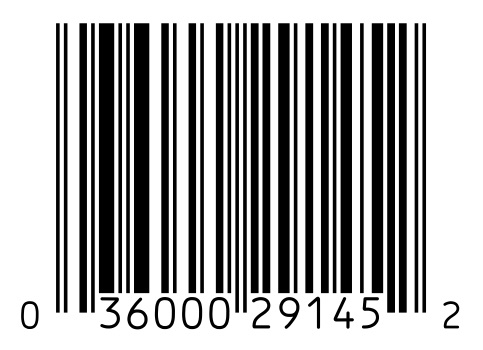
\includegraphics[scale=.5]{Barcode}\end{center}
\end{multicols}
\begin{solution}$10^5=100,000$\end{solution}
\newpage

\question[24] In a recent survey of 884 Americans between the ages
of $18$ and $50$,\\ $120$ reported that they have tattoos,
$72$ have body piercings, and $41$ have both.
\footnote{Source: 2004, American Journal of Dermatology}

\begin{parts}
\part What is the probability that a randomly
selected American has a tattoo?
\begin{solution}[1.5cm]
$\frac{120}{884}\approx 0.136$
\end{solution}
\part What is the probability that a randomly
selected American has a piercing?
\begin{solution}[1.5cm]
$\frac{72}{884}\approx 0.081$
\end{solution}
\part What is the probability that a randomly
selected American has a both a tattoo and a piercing?
\begin{solution}[1.5cm]
$\frac{41}{884}\approx 0.046$
\end{solution}
\part\label{Independent} According to this data do
the decision to get a piercing and the decision
to get a tattoo appear to be independent?
Recall that two events $E$ and $F$ are called {\em independent}
if $P\left(E\right)P\left(F\right)=P\left(E\cap F\right)$.
\begin{solution}[1.5cm]
No, since $0.136\cdot 0.081\approx 0.011\ne 0.046$
\end{solution}
\part What is the probability that a randomly
selected American has a tattoo given that that individual
has a piercing?
\begin{solution}[1.5cm]
$\begin{xy}<.5cm,0cm>:
(-1,2)*+!D{\text{T}};
(1,2)*+!D{\text{P}};
(-1,0)*\cir<1cm>{};
(1,0)*\cir<1cm>{};
(0,0)*{41};
(-2,0)*{79};
(2,0)*{31};
(4,0)*{733};
\end{xy}$
\qquad $\frac{41}{72}\approx 0.569$
\end{solution}
\part What is the probability that a randomly
selected American has a piercing given that that individual
does {\bf not} have a tattoo?
\begin{solution}[1.5cm]
$\frac{31}{31+733}\approx 0.041$
\end{solution}
\end{parts}
\newpage

\question[16] How many anagrams of the word
{\textsf{Machiavellianism}} are there?
\begin{solution}[2in]
The number of times each distinct letter appears is
shown in the following table.
\[\begin{array}{r|cccccccccc}
\text{letter}&a&c&e&h&i&l&m&n&s&v\\\hline
\text{frequency}&3&1&1&1&3&2&2&1&1&1
\end{array}\]
Thus the number of anagrams is
\[\frac{16!}{3!3!2!2!}=145,297,152,000.\]
\end{solution}

\question[16] This question involves the game of farkle.
\begin{parts}
\part\label{SixFives}
What is the probability of rolling six 5's on a single
roll of six dice?
\begin{solution}[1in]
$\frac{1}{6^6}=\frac{1}{46656}\approx 0.00002$\end{solution}
\part What would be the score for the outcome in (\ref{SixFives})?
\begin{solution}[1in]2000\end{solution}
\part What is the probability of rolling {\bf at least one} 5
on a single roll of six dice?
\begin{solution} It's easier to count the ways for the desired
event to fail. Namely, we count the ways to roll {\em no 5's}.
This can occur in $5^6=15625$ ways. Thus the probability
of at least one 5 is $1-\frac{5^6}{5^6}=\frac{31031}{46656}
\approx 0.6651$.
\end{solution}

\end{parts}

\vfill
\begin{center}\gradetable[h][questions]\end{center}

\end{questions}
\end{document}
